\chapter{绪论}

\section{研究背景及意义}

区块链(Blockchain)是一种按照时间顺序将数据区块以链条的方式组成的特定数据结构,被视为一个分布式的共享账本和数据库。它能够使用户无第三方的条件下可信中介的情况下完成可信的价值传输\cite{SurveyofEnterpriseBlockchains}。作为区块链2.0 的以太坊\footnotemark[1]\footnotetext[1]{\href{http://github.com/ethereum/wiki/wiki/White-Paper/}{以太坊白皮书}}重新将智能合约描述为图灵完备的、部署于区块链网络中合同条款代码。这意味着传统的合同条款可以进入实体计算机中,且在区块链网络去中心化、不可伪造、不可篡改的特性下严格执行。区块链推进了人与企业之间和线上与线下的全方面互联,其被成为下一代的新型生产关系。随着区块链的快速发展, 智能合约极大地丰富和扩展了区块链应用场景。它们为供应链、金融等传统领域带来重大变革, 已经快速渗入到人们生活的方方面面。目前, 去中心化应用纷纷落地, 逐步从概念验证阶段转化为工程化实践阶段\footnotemark[2]\footnotetext[2]{\href{https://www.bilibili.com/video/BV1vK4y1A7pY?spm_id_from=333.337.search-card.all.click}{自动化框架 (BAF) 简介}}。

与此同时, 云原生(Cloud native)是一种基于云的软件架构思想和软件开发实践的一组方法论。因其弹性和分布式的优势成为当今流行的软件服务模式。云原生技术有利于各组织在公有云、私有云和混合云等新型动态环境中, 构建和运行可弹性扩展的应用, 借助平台的全面自动化能力, 跨多云构建微服务, 持续交付部署业务生产系统。

区块链即服务(Blockchain as a Service, 简称BaaS)则是基于云原生技术体系的一种构建、管理、托管和运维区块链网络及其应用的云服务平台\cite{onik2019performance}。BaaS支持将任何企业级区块链实施到云环境,而无需任何IT专业知识。这大大降低了区块链技术的使用门槛, 是促使区块链技术更广泛、更深入地渗透到各个行业和企业的催化剂, 其市值预计从2018年的6.23亿美元猛增2023年的150亿美元\footnotemark[3]\footnotetext[3]{\href{https://www.reportbuyer.com/product/5486837/global-blockchain-as-a-service-market.html}{Global Blockchain-as-a-Service Market 2018-2022}}。市场发展迅速, 具有极大的商业价值。其中, 云厂商提供了大多数的BaaS平台\cite{KuernetesbasedFabricChaincodeManagementAndHihgAvailabilityTechnology}, 如表\ref{major_BaaS_platforms}所示, 其底层区块链支撑技术大多数选择IBM开源的跨企业级联盟链Hyperledger Fabric, 这也是本文选择Hyperledger Fabric的原因。

{\footnotesize
\begin{longtable}[h]{m{100pt} m{50pt} m{50pt} m{50pt} m{50pt}}
    \caption[主要公有云的BaaS平台]{主要公有云的BaaS平台} \label{major_BaaS_platforms} \\
        \toprule  
        \textbf{BaaS平台}&\textbf{Ethereum}&\textbf{Quorum}&\textbf{Corda}&\textbf{Fabric}\\
        \hline
        
        AWS&Y&Y&Y&Y\\

        Azure&Y&Y&Y&Y\\

        IBM& & & &Y\\

        阿里云区块链服务&Y& & &Y\\

        腾讯云区块链服务TBaaS& & & &Y\\

        华为云区块链服务BCS& & & &Y\\
        \bottomrule
    \end{longtable}
}



% 挑战
BaaS基于云的自动化的能力屏蔽了底层区块链技术, 为上层去中心化应用的开发运维人员提供便捷的构建区块链网络等功能。然而, “Each coin has two sides”, 当前BaaS平台的发展尤其是底层的区块链基础设施的建设依旧存在诸多挑战。

首先, 基础商业化应用工具并不完善\footnotemark[2]\footnotetext[2]{\href{http://www.caict.ac.cn/kxyj/qwfb/ztbg/202107/P020210726503897354430.pdf}{区块链基础设施研究报告(2021年)}}。BaaS平台发展还处于初级阶段, 商业运行模式仍处在探索阶段。由于BaaS平台研发投入大, 目前市场上存在如AWS、IBM、阿里云区块链服务等多种BaaS平台解决方案, 这些BaaS平台计费高昂\footnotemark[3]\footnotetext[3]{\href{https://help.aliyun.com/document_detail/107710.html?spm=5176.14107623.commonbuy2container.1.59523b20xmyuNf}{阿里云区块链服务BaaS规格与定价}}并且与其他云服务捆绑销售。传统的企业业务或已存在稳定合作的云服务商, 使用不同云服务商的合作伙伴就需要跨云部署, 由于缺乏统一的顶层规划, 各云厂商的BaaS导致不同应用底层异构形成技术、信息孤岛, 存在不可复用的跨解决方案的资源和工具, 这导致了基于多云的网络\cite{DBLP:conf/coins/GerritsKKFV21}, 给跨云部署带来了诸多问题。同时, BaaS平台几乎都由互联网云服务巨头企业把控, 可用性限制通常会迫使其他企业为来自各种云提供商的基础设施即服务(Infrastructure as a Service, 简称IaaS)付费, 最终行业马太效应明显\cite{KuernetesbasedFabricChaincodeManagementAndHihgAvailabilityTechnology}。

其次, BaaS平台利用云能力对区块链基础设施赋能乏力。作为一种广泛部署的技术, 云计算是实施区块链技术的合适目标。然而, 区块链与云原生两种技术都相对不成熟, 但两者的集成可能会在技术方面产生新的复杂性\cite{onik2019performance}。行业缺少既定的标准或最佳实践范例, 各云厂商的BaaS解决方案基本都采取已有的开源解决方案, 业务同质化严重。他们 仅提供一种基于开源区块链平台的自动部署管理方案, 未深入到区块链与云基础设施的底层, 问题仍然在于如何使区块链和云兼容\cite{gai2020blockchain}, 区块链服务比常规云服务更复杂, 有许多未解决的问题需要回答。现有的云厂商BaaS解决方案集中在利用自动化脚本部署区块链网络。然而, 自动化脚本部署并不是有效的云化方式, 浪费了云原生技术的潜力。例如除区块链网络自动部署外, 在数据存储备份及可扩展性方面, 传统自动化部署方案无法利用云的弹性伸缩能力性且随着交易数量的增加, 区块数据最终会占满磁盘空间, 出现存储膨胀问题。区块链的数据可扩展性受到了的限制, 需要结合云的能力寻找数据备份、升级及可扩展性的方法。区块链如何和云原生快速深度结合, 利用原生伸缩性、可移植性和高可用性价值来提供“高质量”的区块链服务, 是当前仍然遗留的挑战。

% 意义、愿景
针对上述问题, 本文选择面向联盟链场景开源框架Hyperledger Fabric和Kubernetes提出了一种区块链云化框架, 具体工作如图\ref{framework_tool}所示。本文首先根据BaaS基础设施存在的挑战结合Kubernetes Operator进行了快速评审, 得到基于Kubernetes Operator云化赋能传统领域的策略集。其次, 结合Hyperledger Fabric网络的特性本文对策略集进行了筛选获得具体云化方案。然后, 基于云化方案, 本文设计了面向Hyperledger Fabric的区块链云化框架。该框架通过对Hyperledger Fabric网络中的Ca、Orderer、Peer组件进行抽象适配并利用Kubernetes Operator对其进行完整生命周期管理。框架利用原生Kubernetes安全性、可扩展性等机制使用户通过专家提供的领域知识对Hyperledger Fabric网络获得类似云的自我管理。最终, 本文还实现了基于区块链云化框架的原型工具, 支持更简单、更原生的管理Hyperledger Fabric网络。

\begin{figure}[h] %figure环境,h默认参数是可以浮动,不是固定在当前位置。如果要不浮动,你就可以使用大写float宏包的H参数,固定图片在当前位置,禁止浮动。
    \centering %使图片居中显示
    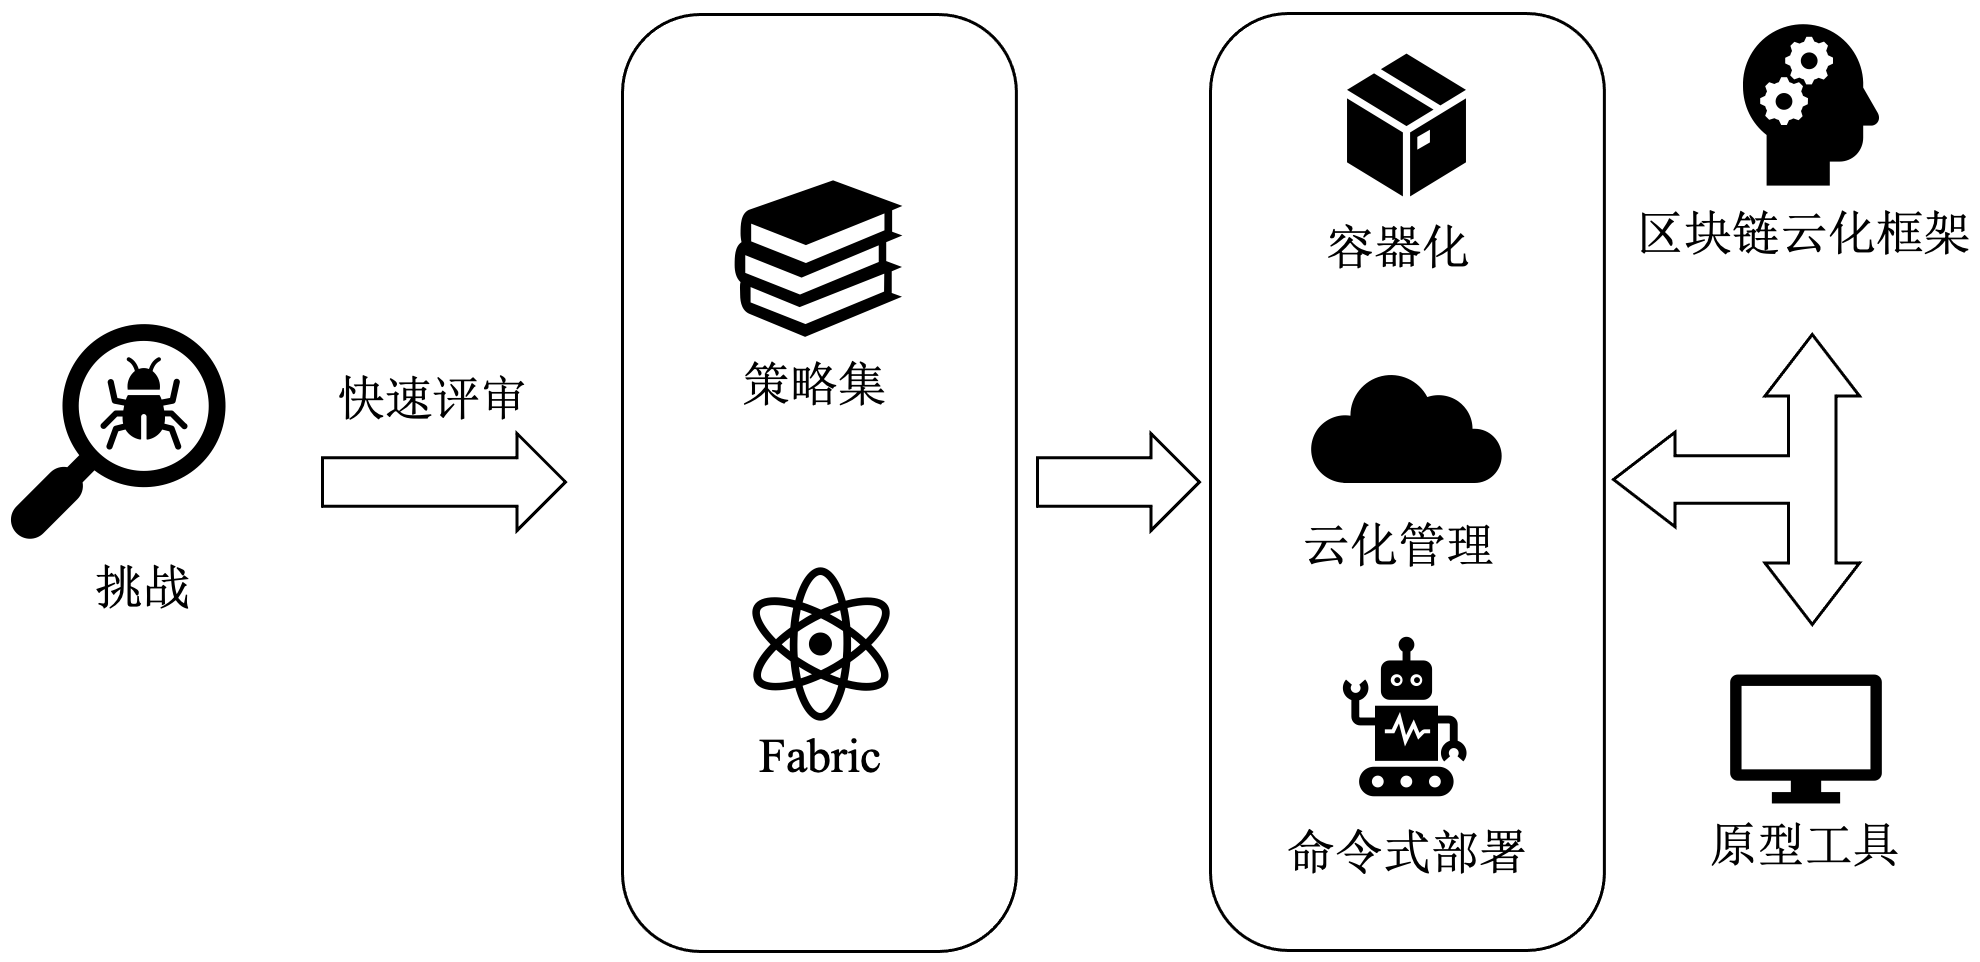
\includegraphics[width=0.85\textwidth]{FIGs/chapter1/process.png} %中括号中的参数是设置图片充满文档的大小,你也可以使用小数来缩小图片的尺寸。
    \caption{区块链云化框架及其原型工具} %caption是用来给图片加上图题的
    \label{framework_tool} %这是添加标签,方便在文章中引用图片。
\end{figure}%figure环境

\section{研究现状}

由于区块链智能合约的无法删除、修改、历史可追溯、去中心化、严格执行等特点, 越来越多的研究人员想挖掘区块链的潜能, 将区块链的能力应用到各种应用场景。McCorry等人\cite{mccorry2017smart}将区块链应用在电子投票领域, 实现了一个基于以太坊的去中心化互联网公开投票协议,公开投票网络是一种自助协议, 每个选民都控制着自己投票的隐私, 只有在所有人都参与的情况下才会被破坏, 这是第一个实现的不依赖任何可信的权威机构来计数和保护选民隐私的去中心化应用。Chang和Chen\cite{chang2020blockchain}在供应链领域进行了系统文献综述,表明传统的供应链活动涉及多个中介、信任和性能问题,利用区块链的潜力可以更好地扰乱供应链运作性能、分布式治理和过程自动化。Zhang和Wen\cite{zhang2017iot}提出了一种物联网电子商务模型,旨在重新设计传统电子商务模型中的许多元素,并借助区块链和智能合约技术在物联网上实现智能财产和付费数据的交易。Leka等人\cite{leka2019systematic}相信区块链技术将是下一个技术革命,同时表明区块链研究现阶段在物联网\cite{christidis2016blockchains}、医疗、教育、政府各个领域都有涉及。

目前, 去中心化应用逐步从概念验证阶段转变为工程化、商业化阶段。由于区块链的复杂性给网络的构建以及智能合约的部署、运维工作带来了严重的时间成本。在去中心化应用价值交付过程中, 存在对于区块链底层技术的易用性、部署效率、安全性等多方面的挑战。研究人员在区块链基础设施与云原生结合方面都开始了一定的探索, 除了利用区块链的特性提升云的能力外\cite{DBLP:journals/comcom/XieZZWH21}\cite{DBLP:conf/smartcloud/SunWY20}\cite{8457813}, 研究人员也都期望利用云的特性自动化地构建出易于弹性扩展、高可用的区块链平台。

% 学术
% 应用场景 BaaS平台往云上迁移
在学术研究方面, 研究人员在探究如何有效利用云平台来部署区块链平台。Gerrits等人\cite{DBLP:conf/coins/GerritsKKFV21}在Kubernetes中部署了分布式账本Hyperledger Sawtooth\footnotemark[1]\footnotetext[1]{\href{https://github.com/hyperledger/sawtooth-core}{Hyperledger Sawtooth github地址}}, 并运行了一个用例。他们旨在探讨该用例在真实场景云部署中的可行性和可扩展性。Liang等人\cite{liangeduchain}针对教育领域数据共享和信息欺骗的问题构建了一个高可用的教育联盟区块链平台, 并实现了基于Kubernetes的Fabric部署, 实现了将链码纳入Kubernetes环境管理的目标。然而, Wan等人\cite{wan2018novel}指出当前主流的BaaS提供商通常采用API进行用户访问, 或者简单地将区块链应用迁移到云, 这会侵蚀不可信的机制并带来锁定风险。他们随后提出了一种新的服务范式来克服现有BaaS的局限性。基于Fabric的实施表明, 该范式可以缓解当前BaaS对区块链特征的侵蚀。在云原生底层基础设施方面研究人员关注与区块链结合的Kubernetes调度问题。才丽\cite{caili2018}在Kubernetes上面对PBFT和区块链的本身特性提出了静态调度和自适应算法。Shi等人\cite{9582270}为了解决云端现实PoS区块链工作负载的高效调度问题, 首次在云计算中设计和实现了基于Kubernetes的解决PoS区块链应用程序迁移成本的系统, 最大限度地减少了使用的Kubernetes工作节点数量以降低总体费用,而且还提出了一种高性能的Kubernetes调度方案HPKS以最大限度地利用工作节点进行在线pod管理。

% 工业界
相比于学术研究, 工业领域的探索更加注重自动化实践。Hyperledger Cello\footnotemark[1]\footnotetext[1]{\href{https://github.com/hyperledger/cello}{Hyperledger Cello}}支持在多种底层基础设施上从头快速构建BaaS平台, 提供管理区块链网络的生命周期、自定义区块链网络配置等功能帮助人们以更高效的方式使用和管理区块链。Hyperledger Cello当前阶段重点关注在Docker安装, 对于Kubernetes支持方面的仍处在相对初级阶段, 配置项简单灵活性不足且老旧。Blockchain Automation Framework\footnotemark[2]\footnotetext[2]{\href{https://github.com/nikoturin/blockchain-automation-framework}{Blockchain Automation Framework}}提供了一个自动化框架, 利用Ansible\footnotemark[3]\footnotetext[3]{\href{https://github.com/ansible/ansible}{Ansible}}以及Helm\footnotemark[4]\footnotetext[4]{\href{https://github.com/helm/helm}{Helm}}快速地、一致地将生产就绪的分布式账本技术(Distributed ledger technology, 简称DLT)平台部署到云基础设施。虽然, Blockchain Automation Framework提供了一个自动化框架将区块链平台部署于Kubernetes, 但本质上还是描述为一个需要希望远程主机执行命令的方案,或者一组IT程序运行的命令集合。这大大提升了自动化程度,但其远没有发挥Kubernetes的潜力。

% 总结
尽管学术界以及工业界目前已有一些关于区块链云化的探索与研究, 但研究重点多为如何自动化地将区块链平台向云上迁移, 并且区块链平台的性能往往由于许多影响因素而不稳定, 尤其是当它们部署在动态云环境中的时候。当前研究缺少构建支持云和区块链一体化的有效服务模型\cite{9582270}, 所以需要在云中操作区块链的实证研究\cite{8790849}。

在云中操作应用程序就需要将应用程序部署进Kubernetes, 这个过程需要部署多种资源, 如Deployment、Service等。虽然这些资源有标准定义的模板只需要在不同程序上定义不同的参数, 但目前用户人为创造定义这些资源会导致大量重复的代码并引入人为错误, 错误的资源定义会直接影响Kubernetes中应用程序的工作。Kubernetes Operator是将领域知识集成到Kubernetes API编排过程中的最新方法\cite{henning2021reproducible}。一部分研究利用Kubernetes Operator方法通过自动化的方式将云底层的效率、灵活性等多方面优势拓展到多种领域。Huang等人\cite{huang2021fly}提出了一个轻量级的遥感大数据处理云原生框架。该框架利用Kubernetes Operator融合Spark, 自动化配置Spark参数, 提升并行遥感图像融合算法的效率。Zhou等人\cite{zhou2021container}提出了Torque operator对高性能(High Performance Computing, 简称HPC)的负载进行管理, 利用容器化来提升HPC的效率及灵活性。除此之外, 在5G领域\cite{arouk20205g}\cite{wiranata2020automation}、医疗\cite{rouzbeh2020unified}等领域, Kubernetes Operator也发挥出其强大的自动化与编排能力, 利用云原生的可迁移性、可伸缩性、安全性等特性进行赋能, 但在区块链领域的Kubernetes Operator相关工作较少。


\section{本文主要研究工作}

本文的主要研究工作分为以下三个方面: 

1. 本文首先基于当前BaaS平台存在的挑战结合Kubernetes Operator进行了快速评审。快速评审的范围涵盖了计算机与软件工程领域的权威全文数据库。经过快速评审, 本文得到了12条Kubernetes Operator赋能传统领域提升软件质量属性的策略集。根据区块链云化设计原则, 结合区块链网络的特性, 最终形成了区块链云化具体实施方案。

2. 基于上述具体实施方案, 本文设计实现了面向Hyperledger Fabric的区块链云化框架及其原型平台。框架为Fabric网络编写三种用户自定义资源(Custom Resource Defination, 简称CRD), 包含Ca、Peer、Orderer。这些CRDs将区块链领域知识注入Kubernetes基础设施, 通过这种方式可以自动化配置网络, 消除人为错误, 提升云化框架的易用性。其次, Manager作为框架中枢处理单元对利用Helm对Hyperledger Fabric网络中的节点进行全生命周期管理, 并根据实施方案, 复用Kubernetes原生手段提升框架及Hyperledger Fabric网络的可扩展性、安全性以及可视运维的能力。最后, Hyperledger Fabric网络作为框架的输出单元, 包含了维持Hyperledger Fabric网络节点运行的各种配置以及合理的运行状态。

3. 本文对原型平台进行了测试与评估。以典型案例的方式对原型工具进行了功能性与非功能性测试, 通过五层成熟度模型对原型工具进行了定性评估, 通过与Hyperledger官方的BaaS工具Cello对比进行了定量评估。结果表明, 本文的原型工具在兼容基本BaaS功能的前提下能够充分利用云的特性提升Fabric网络及其节点的数据可扩展性、安全性以及可视运维的能力, 本文的原型工具可以基本满足五层成熟度模型的能力, 并且在网络部署时间方面, 原型工具具有更优且更稳定的表现。


\section{本文组织结构}

本文组织结构如下:

第一章~绪论。介绍了本文的研究背景及意义、国内外研究现状、工业界的主要探索以及本文主要的研究工作。

第二章~理论与技术支持。介绍区块链尤其是Hyperledger Fabric的相关理论和概念; 同时介绍云原生的基本概念发展历程, 并对云原生基础设施Kubernetes进行了详细介绍。

第三章~区块链云化框架调研与分析。介绍通过快速评审获得Kubernetes Operator赋能传统领域的策略集, 同时结合区块链云化设计原则以及区块链本身特性对策略集进行筛选得到具体云化实施方案。

第四章~基于Hyperledger Fabric的区块链云化框架。介绍了本文提出的基于Hyperledger Fabric的区块链云化框架, 包含输入、处理以及输出单元; 介绍了原型工具的需求分析、设计与实现。

第五章~测试与评估。以典型案例分析的方式对原型工具进行功能性与非功能性测试; 对原型工具进行定性与定量评估。

第六章~总结与展望。对全文进行总结; 阐述了区块链云化框架的局限性; 对未来工作进行展望。


